\subsection{Карта режимов}

    Карта режимов, представленная на рисунке \ref{regimeMap}, позволяет показать возникающие динамические режимы системы при определенных значениях параметров \(\alpha\) и \(\beta\).

    Можно заметить, что при любом значении параметра \(\alpha\) существует каскад бифуркации удвоения периода при уменьшении параметра \(\beta\). Чем меньше параметр \(\alpha\), тем меньше интервал значений параметра \(\beta\), при котором этот каскад существует. После его исчезновения аттрактором системы является равнвовесие \(\bar{x}_1\).

    \begin{figure}
        \centering
        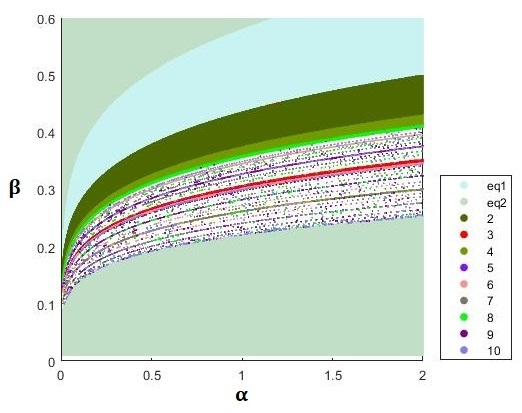
\includegraphics[width=\textwidth]{deterministic/images/regime_map.jpg}

        \captionsetup{justification=centering}
        \caption{Карта режимов модели (\ref{origin})}
        \label{regimeMap}
    \end{figure}
